\documentclass[a4paper]{article}

\input ../header
\usepackage{minted}
\usepackage[np]{numprint}
\usepackage{lscape}
\usepackage{afterpage}
\usepackage{hyperref}

\setlength{\multicolsep}{2pt}

\begin{document}

\title{Le réseau Internet (première partie)}

\pagestyle{empty}

\date{}
\author{}

\maketitle{}

\thispagestyle{empty}
\noindent\textbf{Activité 1}\hfill{}\textbf{Introduction}
\smallskip
\hrule
\smallskip

\begin{enumerate}
  \item Chercher une définition du réseau Internet (4 à 5 phrases).
  \item Y a-t-il une différence entre le Web et Internet ?
  \item Citer plusieurs services proposés par le réseau Internet.
\end{enumerate}

\bigskip

\noindent\textbf{Activité 2}\hfill{}\textbf{Quelques repères historiques}
\smallskip
\hrule
\medskip

En utilisant l'outil de votre choix, réaliser une frise chronologique décrivant la naissance du réseau Internet et son évolution. La déposer sur Moodle.
On pourra faire figurer, entre autres, les repères historiques suivants :
% Dates et références dans le livre jaune SNT (éditions Ellipses)
\begin{itemize}
  \item invention du modem;
  \item création d'{\color{red}Arpanet};
  \item envoi du premier courrier électronique;
  \item création du {\color{red}réseau Cyclades};
  \item abandon du projet Cyclades;
  \item création du {\color{red}DNS};
  \item création de {\color{red}Napster};
  \item naissance du World Wide Web;
  \item arrivée du navigateur {\color{red}NCSA Mosaic}.
\end{itemize}

Rechercher la définition/expliquer les mots écrits précédemment en rouge (deux ou trois phrases par mot).

\bigskip

\noindent\textbf{Activité 3}\hfill{}\textbf{Les câbles sous-marins}
\smallskip
\hrule
\medskip

\begin{enumerate}
  \item Regarder les vidéos disponibles sur Moodle puis faire le test proposé.
  \item Trouver une carte des câbles sous-marins.
  \item Combien de câbles arrivent en Polynésie ? Comment se nomment-ils ?
  \item Préciser la date de pose et la longueur de chacun des câbles précédents.
  \item Quelles îles permettent-ils de relier ?
\end{enumerate}

\bigskip


\noindent\textbf{Activité 4}\hfill{}\textbf{Ordre de grandeur}
\smallskip
\hrule
\medskip

\begin{enumerate}
  \item Qu'est-ce qu'un bit ? un octet ?
  \item Quelle est la traduction anglaise d'un octet ?
  \item Qu'est-ce qu'un mégaoctet (Mo) ? un gigaoctet (Go) ? un téraoctet (To) ?
  \item Compléter le graphique suivant qui décrit l'évolution du volume mensuel de trafic sur Internet entre 2017 et 2022.\\
    \textit{Indication. -- En utilisant un moteur de recherche, chercher par exemple \og{}Cisco Visual Networking Index\fg{}.}

%    \begin{minted}{python}
%      import matplotlib.pyplot as plt
%
%      annees = range(2017, 2023)
%      trafic = [0, 0, 0, 0, 0, 400]
%      trafic2 = [122, 0, 0, 0, 0, 0]
%      # trafic_complet = [122, 156, 201, 254, 319, 396]
%      plt.bar(annees, trafic, width=0)
%      plt.bar(annees, trafic2, width=0.5, color='lightgreen')
%      plt.grid(axis='y')
%      plt.title('Volume mensuel de trafic sur Internet\n En exaoctets')
%      plt.text(2016.83, 100, "122")
%      plt.savefig('trafic.png')
%    \end{minted}

    \begin{center}
      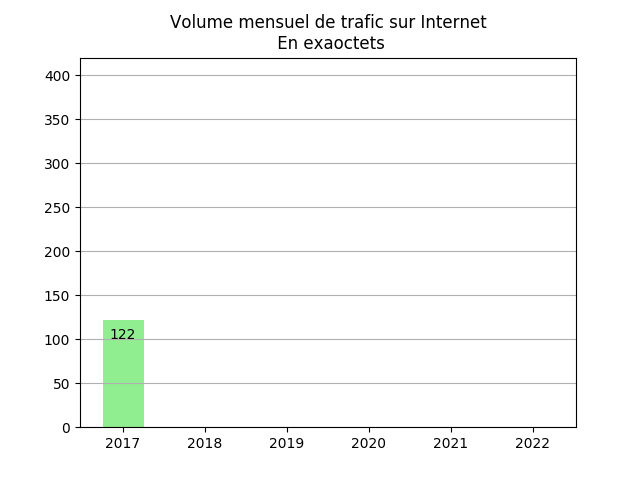
\includegraphics[width=10cm]{trafic.png}
    \end{center}
  \item Que signifie le nombre $\np{122}$ du graphique précédent ?
  \item Expliquer comment retrouver approximativement la valeur $\np{150700}$ gigaoctets/seconde du tableau suivant à partir des données de la question précédente.
    \begin{center}
      \renewcommand{\arraystretch}{1.2}
      \begin{tabular}{|>{\centering}m{2cm}|>{\centering}m{5cm}|}
	\hline
	Années & Trafic Internet global\tabularnewline
	\hline
	1992 & $100$ gigaoctets/jour\tabularnewline
	\hline
	1997 & $100$ gigaoctets/heure\tabularnewline
	\hline
	2002 & $100$ gigaoctets/seconde\tabularnewline
	\hline
	2007 & $\np{2000}$ gigaoctets/seconde\tabularnewline
	\hline
	2017 & $\np{46600}$ gigaoctets/seconde\tabularnewline
	\hline
	2022 & $\np{150700}$ gigaoctets/seconde\tabularnewline
	\hline
      \end{tabular} 
    \end{center}
  \item Dans cette question, on considèrera que :
    \begin{itemize}
      \item un disque dur de capacité $2$ To a la forme d'un parallélépipède rectangle de dimensions $10$ cm, $15$ cm et $2,5$ cm ;
      \item qu'une salle de classe a une superficie de $50$ m$^2$ et une hauteur de $3$ m.
    \end{itemize}
    À quel nombre de salles de classe remplies avec des disques durs de $2$ To correspond le volume quotidien échangé sur Internet en 2022 ?
\end{enumerate}

\bigskip

\noindent\textbf{Activité 5}\hfill{}\textbf{Un peu de Python}
\smallskip
\hrule
\medskip

\begin{enumerate}
  \item Le module pyplot de la bibliothèque Matplotlib permet de construire toutes sortes de graphiques en utilisant Python. Créer un notebook Jupyter vide, puis essayer le code suivant dans une cellule :

    \bigskip

    \begin{minted}{python}
      import matplotlib.pyplot as plt

      annees = [2017, 2018, 2019, 2020, 2021, 2022]
      volume = [122, 156, 201, 254, 319, 396]
      plt.bar(annees, volume, width=0.5, color="lightblue")
      plt.grid(axis="y")
      plt.title("Volume mensuel de trafic sur Internet en exaoctets par mois")
      # plt.show()
    \end{minted}

  \item Décommentez la ligne 8, puis réessayer le code.
  \item Ajouter les lignes suivantes, puis essayer encore une fois :

      \begin{minted}{python}
      plt.xlabel("Années")
      plt.ylabel("Volume mensuel en exaoctets")
      \end{minted}
  \item Expliquer alors chaque ligne du code précédent.
  \item Comment obtenir le graphique suivant ?
    \begin{center}
      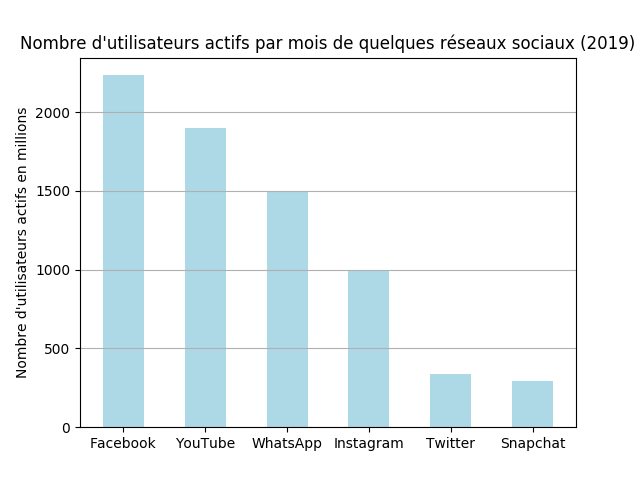
\includegraphics[width=10cm]{utilisateurs_actifs_reseaux_sociaux.png}
    \end{center}
    \begin{center}
      \renewcommand{\arraystretch}{1.2}
      \begin{tabular}{|>{\centering}m{4cm}|*{6}{>{\centering}m{1.6cm}|}}
	\hline
	Réseau social & Facebook & YouTube & WhatsApp & Instagram & Twitter & Snapchat\tabularnewline
	\hline
	Nombre d'utilisateurs actifs par mois, en millions (2019) & $\np{2234}$ & $\np{1900}$ & $\np{1500}$ & $\np{1000}$ & $\np{335}$ & $\np{291}$\tabularnewline
	\hline
      \end{tabular}
    \end{center}
\end{enumerate}

\noindent\textbf{Activité 6}\hfill{}\textbf{\og{}Tout\fg{} Netflix en une seconde}
\smallskip
\hrule
\medskip

\begin{enumerate}
  \item Lire l'article suivant :
    \begin{center}
      \url{https://www.whats-on-netflix.com/news/how-long-would-it-take-to-watch-all-of-netflix/}
    \end{center}
    Retrouver, par un calcul, la valeur de \og{}$\np{36000}$ heures\fg{} de contenu disponibles sur Netflix (US).
  \item Lire l'article suivant :
    \begin{center}
      \url{https://help.netflix.com/fr/node/87}
    \end{center}
    Quelle quantité de données est consommée lorsqu'on regarde une heure de contenu en haute définition (HD) ?
  \item Récemment, en utilisant de nouveaux amplificateurs, des chercheurs ont pu atteindre une vitesse de transmission de données sur Internet de $178$ Térabits par seconde.
    \begin{enumerate}
      \item Convertir cette vitesse en Gigabits par seconde.
      \item À cette vitesse, combien de temps prendrait le téléchargement du contenu de Netflix (US) en haute définition ?
    \end{enumerate}
  \item Quel est le débit maximal (théorique) proposé par Vini à ses abonnés (particuliers) ? Par combien faudrait-il multiplier cette vitesse pour atteindre les $178$ Térabits par seconde ?
\end{enumerate}

\end{document}
